
\documentclass[sigconf]{acmart}

\usepackage{wrapfig}

\usepackage[english]{babel}

\usepackage{biblatex}

\usepackage{listings}

\setcopyright{none}

\settopmatter{printacmref=false} % Removes citation information below abstract
\renewcommand\footnotetextcopyrightpermission[1]{} % removes footnote with conference information in first column
\pagestyle{plain} % removes running headers
  
\begin{document}
\lstset{language=Python}
  
\title{\HUGE{\textbf{Traind AI Warfleet}}}

\author{Michel Schwarz}
\affiliation{\institution{Hochschule Düsseldorf}}
\email{michel.schwarz@study.hs-duesseldorf.de}

\author{Niklas Tluk}
\affiliation{\institution{Hochschule Düsseldorf}}
\email{niklas.tluk@study.hs-duesseldorf.de}

\begin{abstract} % https://libguides.rhul.ac.uk/referencing/latex
The game War Fleet is a timeless classic, popular to this day in its countless iterations, ranging from the original board game to traditionel video games and more recently VR applications. This is an implementation of said game in Python using neural networks and reinforcment learning (RL). The A2C and PPO2 RL algorithems were employed to train intelligent agents, based on the OpenAI Gym toolkit and the OpenAI Baselines framework, to competently play it.
\end{abstract}
  
\begin{CCSXML}
<ccs2012>
   <concept>
       <concept_id>10010147.10010257.10010258.10010261</concept_id>
       <concept_desc>Computing methodologies~Reinforcement learning</concept_desc>
       <concept_significance>100</concept_significance>
       </concept>
   <concept>
       <concept_id>10010147.10010257.10010282.10010291</concept_id>
       <concept_desc>Computing methodologies~Learning from critiques</concept_desc>
       <concept_significance>100</concept_significance>
       </concept>
   <concept>
       <concept_id>10010147.10010178.10010219.10010221</concept_id>
       <concept_desc>Computing methodologies~Intelligent agents</concept_desc>
       <concept_significance>100</concept_significance>
       </concept>
   <concept>
       <concept_id>10010147.10010257.10010293.10010294</concept_id>
       <concept_desc>Computing methodologies~Neural networks</concept_desc>
       <concept_significance>100</concept_significance>
       </concept>
 </ccs2012>
\end{CCSXML}

\ccsdesc[100]{Computing methodologies~Reinforcement learning}
\ccsdesc[100]{Computing methodologies~Learning from critiques}
\ccsdesc[100]{Computing methodologies~Intelligent agents}
\ccsdesc[100]{Computing methodologies~Neural networks}

%% Keywords. The author(s) should pick words that accurately describe
%% the work being presented. Separate the keywords with commas.
\keywords{intelligent systems, intelligent agents, deep reinforcment learning, neural networks}

%% A "teaser" image appears between the author and affiliation
%% information and the body of the document, and typically spans the
%% page.
\begin{teaserfigure}
 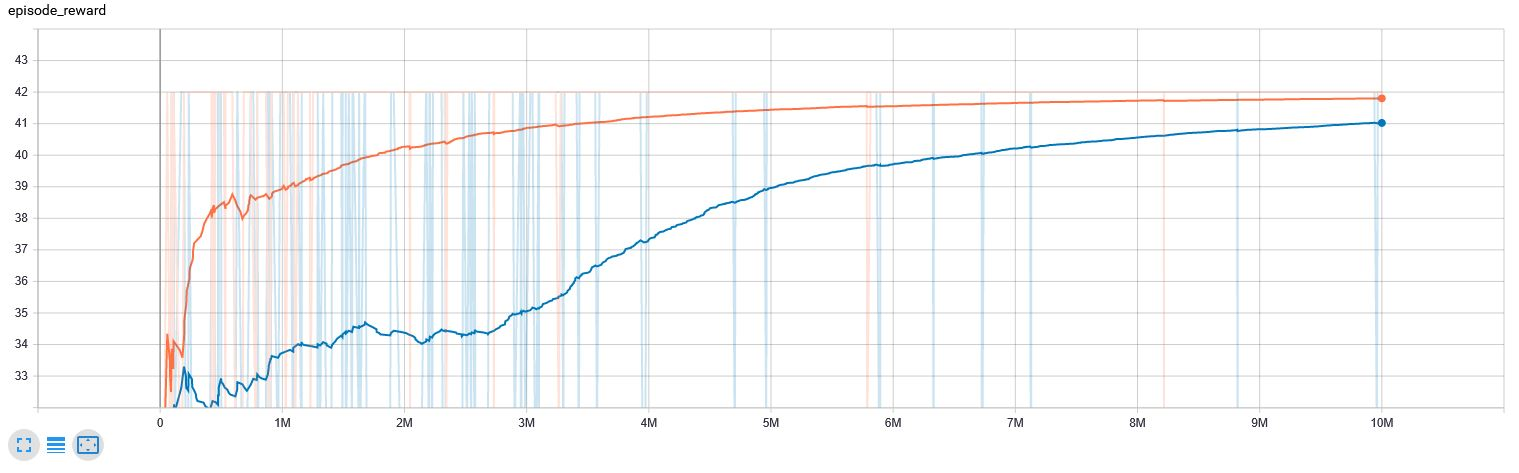
\includegraphics[width=\textwidth]{episode_reward_big} %placeholder
  \caption{Episode Rewards A2C(Orange) and PPO2(Blue).}
  \Description{Enjoying the baseball game from the third-base
  seats. Ichiro Suzuki preparing to bat.}
  \label{fig:teaser}
\end{teaserfigure}

%%
%% This command processes the author and affiliation and title
%% information and builds the first part of the formatted document.
\maketitle 

\section{Introduction}
Considering the current prevalence of machine and deep learning instelligent systems are now more relevent than ever.
This project is part of our participation in the intelligent systems course at the HSD in Düsseldorf, Germany. The course served as an introduction to the design and implementation process of intelligent systems. It contained the history of machine learning, basic underlying principels, methods and algrithems aswell as current relevent topics in the media inforamtics field, like deep leanring, date mining and predictive analytics. 
  
\section{Motivation}
Before starting this course we had already heard  about Deepmind's and OpenAI's impressive and at times even mind-boggling accomplishments with AlphaGO, AlphaStar, OpennAI Five and such. So when we were given the option to train an agent to play a simple game, using reinforcment learning and neural networks, ourselves we were excited and eagerly began coming up with ideas.


\section{Goal}
 Our goal was the training of multiple intelligent agents, capable of competently playing the board game warfleet, in python using reinforcement learning based on the implementation and employment of different models and algorithems. 

\section{Environment}
To achieve this we also had to develop a feasible environment for the agent to be trained in. For this purpose we chose the OpenAI Gym toolkit, which provides an easy-to-use suite of reinforcement learning tasks.
The playing field or board of our game is a 10 by 10 2D array of the type integer. Possible values here are 1 for water, 2 for sections of a ship and 3 for shot positions(impacts).
 ...\\
 ...\\
 ...\\
 ...\\
 ...\\


\vspace{5mm} %5mm vertical space

\begin{wrapfigure}{r}{}
 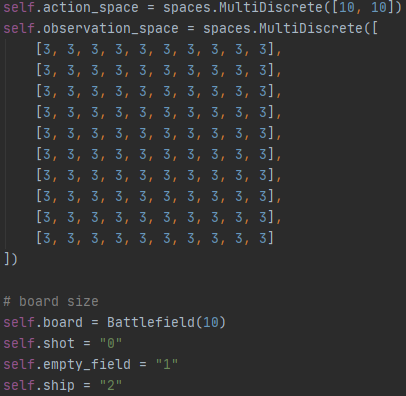
\includegraphics[width=40mm]{spaces.png}
  \caption{Game Board, Observation and Action Space.}
  \Description{...}
  \label{fig:spaces}
\end{wrapfigure}

The action space in our environment consists of all possible coordinates in said board while the observation space describes the amount of possible values, 3 in this case, for every board position.

\vfill %fills remaining section space with blank lines

\section{Methods}
 agents, training, tests
\\
\\
\\
\\
\\
\\
\\
\\
\\
\\
\\
\\
\\
\\
\\
\\
\\
\\
\\
\\


\section{Implementation}
 libs, toolboxes, algs etc.
\\
\\
\\
\\
\\
\\
\\
\\
\\
\\
\\
\\
\\
\\
\\
\\
\\
\\
\\
\\
\\
\\
\\
\\
\\
\\
\\
\\
\\
\\
\\
\\
\\
\\
\\
\\
\\
\\
\\
\\
\\
\\
\\
\\
\\
\\
\\
\\
\\
\\
\vfill %fills remaining section space with blank lines

\begin{figure*}
 \centering
  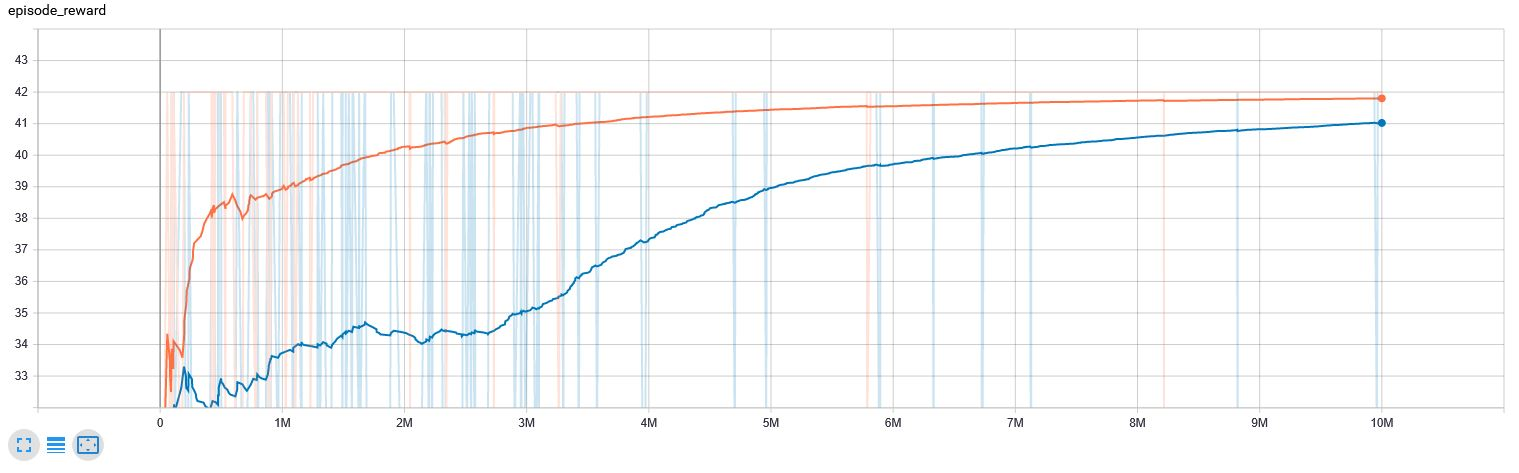
\includegraphics[width=\textwidth]{episode_reward_big} 
  \caption{Episode Rewards A2C(Orange) and PPO2(Blue).}
  \label{fig:reward1}
\end{figure*}

\\

 \section{Results}
 The aforementioned training process resulted in the creation of multiple agents based on both aglorithems. Through prolonged training the agents gained proficiency in playing the game, surpassing the random AI and finally reaching a win rate of 100\% with a varying number of its own ships remaining.
 \\
 \\
This is the end state of a War Fleet game played by the well trained ``a2c\_wp\_2 agents'' against a random AI:

\begin{lstlisting}
--- Computer Battlefield ---
[0, 1, 0, 1, 0, 0, 0, 0, 0, 0]
[1, 1, 1, 1, 1, 1, 1, 1, 1, 1]
[0, 0, 0, 1, 0, 1, 1, 0, 0, 1]
[0, 0, 0, 1, 0, 0, 0, 0, 1, 1]
[1, 0, 1, 1, 0, 0, 0, 0, 1, 1] 
[0, 0, 1, 1, 0, 0, 0, 0, 1, 1] 
[0, 0, 0, 1, 0, 0, 1, 0, 0, 0] 
[0, 0, 0, 1, 0, 1, 1, 0, 1, 1] 
[0, 0, 0, 1, 1, 1, 1, 0, 0, 1] 
[1, 0, 0, 1, 0, 0, 0, 1, 0, 1] 
\end{lstlisting}
\\
\\
As you can see on the computer's battlefield, all of the its ships have been destroyed by our agent quite accuratly with very little shots missing their mark .
\begin{lstlisting}
--- Player/Agent Battlefield ---
[0, 0, 0, 1, 1, 0, 0, 0, 1, 1]
[2, 2, 2, 0, 2, 0, 0, 1, 0, 1]
[0, 0, 0, 0, 1, 1, 0, 0, 0, 0] 
[1, 0, 1, 0, 0, 0, 1, 0, 0, 2]
[0, 0, 1, 2, 0, 0, 0, 2, 2, 2]
[0, 1, 0, 0, 0, 0, 0, 0, 0, 0]
[1, 0, 0, 2, 2, 1, 1, 1, 0, 0]
[0, 0, 0, 0, 2, 0, 0, 0, 0, 0]
[0, 0, 0, 0, 1, 0, 0, 0, 1, 0]
[0, 0, 0, 1, 1, 0, 0, 2, 0, 0]
\end{lstlisting}
Meanwhile the computer, with its random choices, didn't fare nearly as well. It only managed to sink 2 of our agents's ships, mostly just firing at the open water.
\\
\begin{lstlisting}
------------- End -------------
The Agent has won the game
Remaining Ships Computer: 0
Remaining Ships Agent: 8
Reward: [42.] /42
Turns: 121
\end{lstlisting}
\\
With 8 remeaning vessels our agent has bested its opponent in 121 turns, gaining a full reward of 42 points.
\\

\begin{wrapfigure}{r}{}
 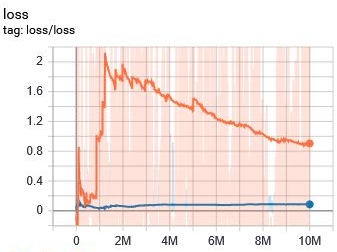
\includegraphics[width=35mm]{loss.png}
  \caption{Loss}
  \label{fig:loss}
\end{wrapfigure}
Figure x1 shows a comparision of one agent of each type after a prolonged training of 10 million timesteps.  It appears that the A2C based agent (a2c) learned very rapidly up to a certain point and than steadily improved over time more slowly while the PPO2 model (ppo2) slowly ramped up over time eventually reaching a steady rate of improvment and slowing down again when approaching the maximum possible reward. After only about 500.000 steps our A2C based model already earned a reward of around 38-39. Meanwhile our PPO2 agent was only able to again a reward of ~33 points.
\\
\begin{wrapfigure}{r}{}
 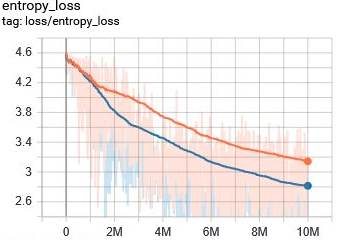
\includegraphics[width=35mm]{eloss.png}
  \caption{Loss}
  \label{fig:loss}
\end{wrapfigure}
At around 1.8 million time steps a2c came in with an average reward of abiut 40 points, thereafter steadily nearing the maximum reward of 42 points, while it took ppo2 around 6.5 million steps the achieve thhe same average.
\\
\\
\begin{figure*}
 \centering
  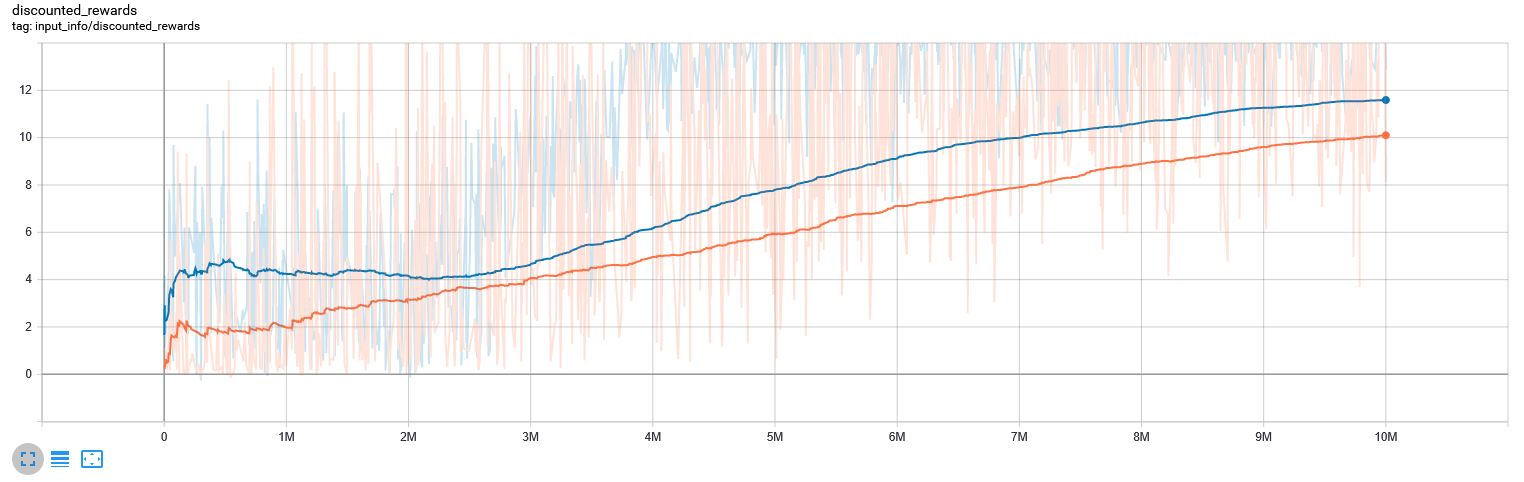
\includegraphics[width=\textwidth]{discounted_reward} 
  \caption{Discounted Rewards A2C(Orange) and PPO2(Blue).}
  \label{fig:reward2}
\end{figure*}

With the reward per episode(figure x1) and the discounted reward (figure x2) connstantly increasing the loss (figure y1) and the entropy loss (figure y2) for a2c deminished over time after first spicking to a starting value of 2.1 und 4.5 respectidly. While the entropy loss of ppo2 also decreased with further training its loss hovered at a value of ~0.1.



\section{Conclusion}
 From those results we can conclude that our A2C based model is more suitable to our environment and was therefore able to gain a greater proficency at plaing the game than our PPO2 based approach at a rapid pace. 
  
\section{Future Work}
Currently there are no plans for further development, with leaves the future of  this project as uncertain. Some possible aproaches are as follows. 
Differnt types of agents wiith varying amounts of training could be put up against each other to display the differnences in learning efficency etc. An option for users to face of against their trained agents could also be implemented.

\end{document}
